\section{Verificaciones}

En esta sección se va a justificar mediante las simulaciones necesarias que el funcionamiento del circuito es el correcto.
Primero, se comprueba que la tensión de salida sin carga es igual a la esperada. En la figura \ref{Vout_50hz} se puede ver que, al transcurrir
un tiempo de aproximadamente $5s$, la tensión de salida se estabiliza en $3101V$, valor que supone un error mínimo del $0,33\%$
respecto a la tensión de salida esperada sin carga ($3111,27V$), como se puede ver en la siguiente expresión:

\begin{equation}
    E_{V_{noload}} = \frac{3111,27V - 3101V}{3111,27V} \cdot 100 = 0,33\%
\end{equation}

\begin{figure}[H]
    \centering
    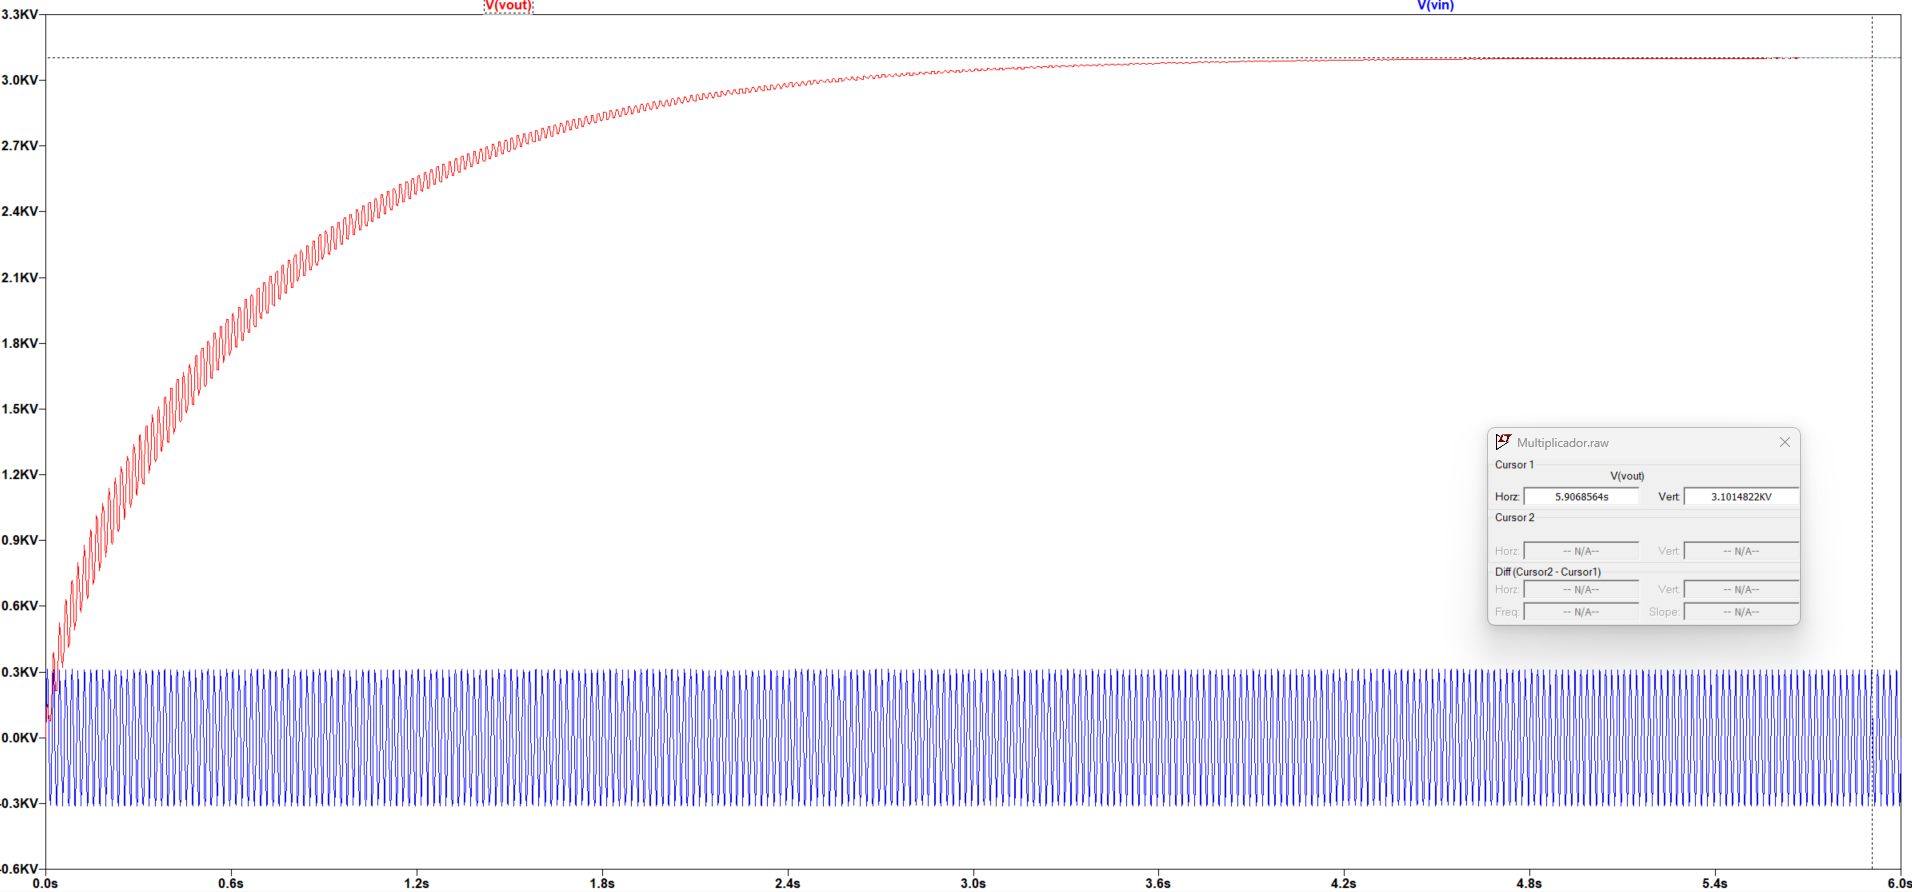
\includegraphics[width=1\textwidth]{Imagenes_alvaro/Vout_50hz.png}
    \caption{Tensión de salida y entrada a $50Hz$ (sin carga)}
    \label{Vout_50hz}
\end{figure}

Además, podemos garantizar que la tensión obtenida está dentro del rango de tensión de salida especificado, puesto que la tensión máxima 
establecida ($5\%$ de $3kV$) es de $3150V$.

Tras comprobar que el circuito funciona correctamente, pasamos a conectar la carga y el circuito de medida.
Respecto del caso anterior, el tiempo de establecimiento es similar y no relevante puesto que no existe ningún requerimiento respecto del mismo, por lo que
se pasa a analizar la tensión de salida en estacionario, obteniendo el resultado \ref{Vout_50hz_load}.

\begin{figure}[H]
    \centering
    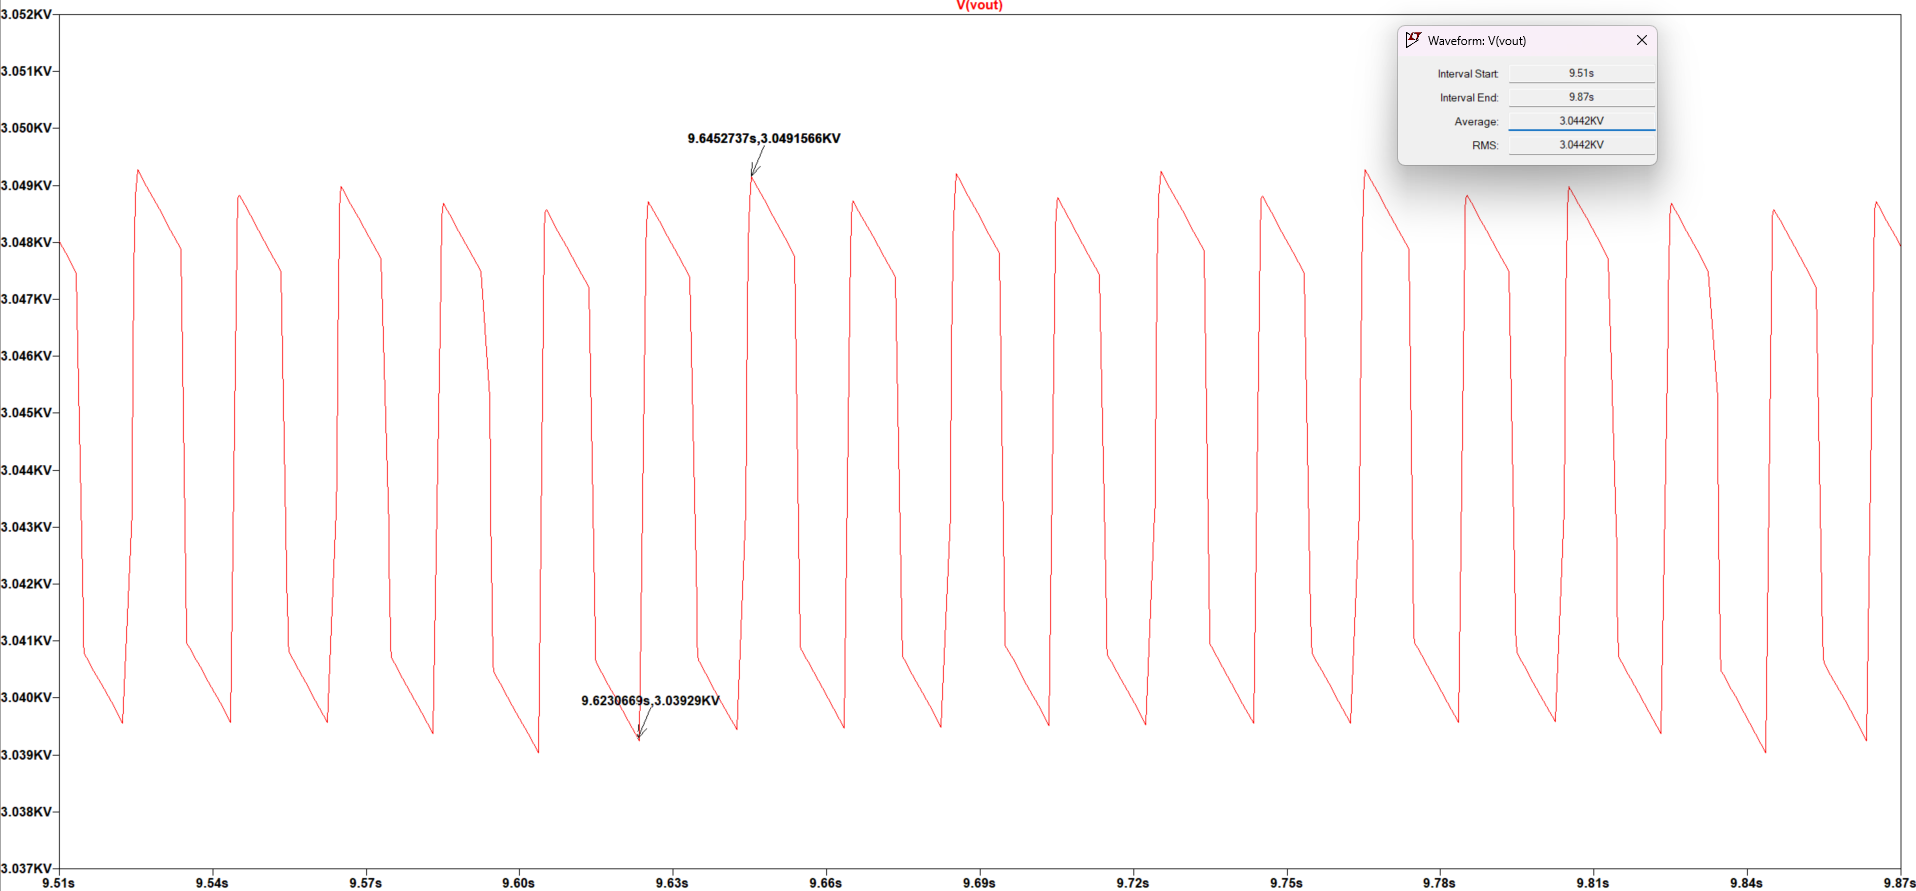
\includegraphics[width=1\textwidth]{Imagenes_alvaro/Vout_50hz_load.png}
    \caption{Tensión de salida a $50Hz$ con carga}
    \label{Vout_50hz_load}
\end{figure}

Como se puede ver en la figura \ref{Vout_50hz_load}, se obtiene una tensión media de $3044V$, una tensión máxima de $3049V$ y una tensión
mínima de $3039V$. De esta manera, se puede garantizar que el requisito de rizado de $10V$ para $50Hz$ sí se cumple, y el error obtenido 
para la tensión media es mínimo:

\begin{equation}
    E_{V_{load}} = \frac{3047,93V - 3044V}{3047,93V} \cdot 100 = 0,13\%
\end{equation}

Respecto a la corriente, se analiza en la figura \ref{Corrientes} la corriente que circula a través de la carga y la que circula a través del circuito
de medida. Puesto que, como se explica en la sección anterior, la tensión de salida es ligeramente menor a la esperada, en consecuencia la corriente en la carga también lo será,
midiendo un valor de $4.898mA$. La corriente a través del circuito de medida se ha diseñado para no ser significativa, dando un valor de $21,718\mu A$.
Se analiza el error cometido en la corriente a través de la carga y del circuito de medida:

\begin{equation}
    E_{I_{load}} = \frac{5mA - 4,898mA}{5mA} \cdot 100 = 2,04\%
\end{equation}

\begin{equation}
    E_{I_{meas}} = \frac{22,22\mu A - 21,718\mu A}{22,22\mu A} \cdot 100 = 2,26\%
\end{equation}

\begin{figure}[H]
    \centering
    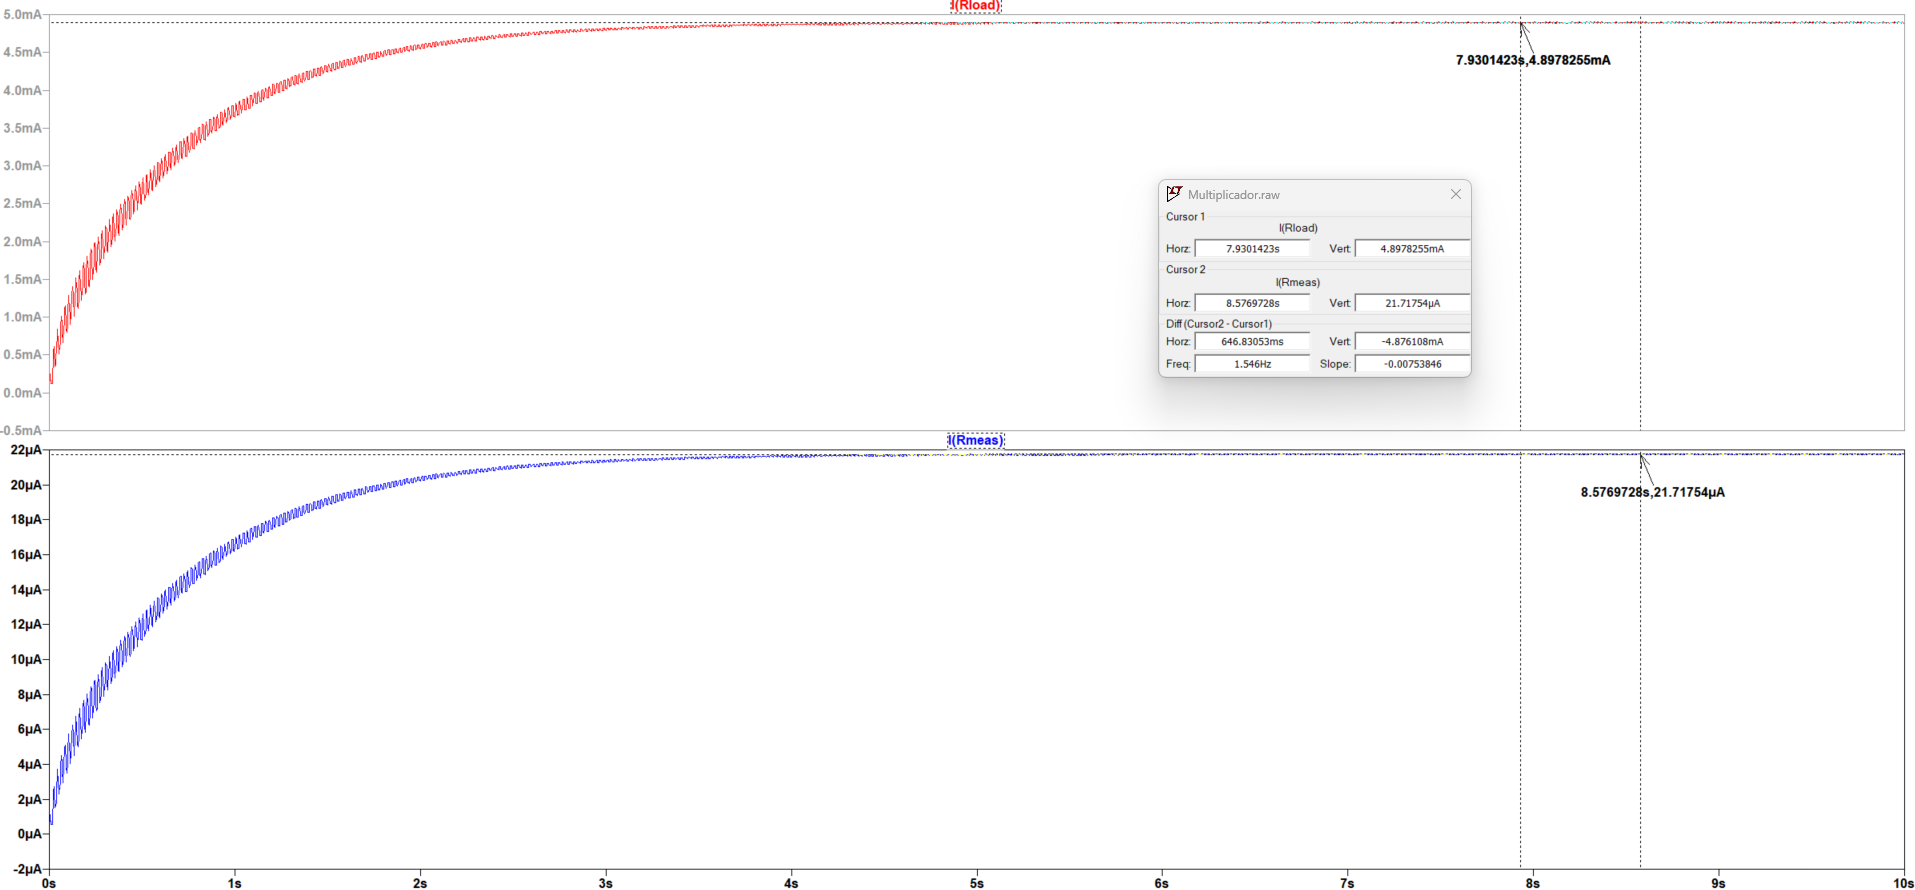
\includegraphics[width=1\textwidth]{Imagenes_alvaro/Corrientes.png}
    \caption{Corriente en la carga y sistema de medida}
    \label{Corrientes}
\end{figure}

Por otra parte, también es necesario analizar la tensión máxima en los semiconductores y condensadores, cuyo resultado se puede ver en la figura \ref{Vmax}.
La tensión máxima es de $618,33V$ (aproximadamente el doble a la de la fuente), mucho menor a los $1000V$ 
establecidos como máximo, por lo que este requerimiento está cumplido. Además, cabe destacar que el primer 
condensador ($C_1$) se carga a una tensión igual a la de la fuente, por lo que se puede utilizar un condensador de menor rango de tensión para este caso.

\begin{figure}[H]
    \centering
    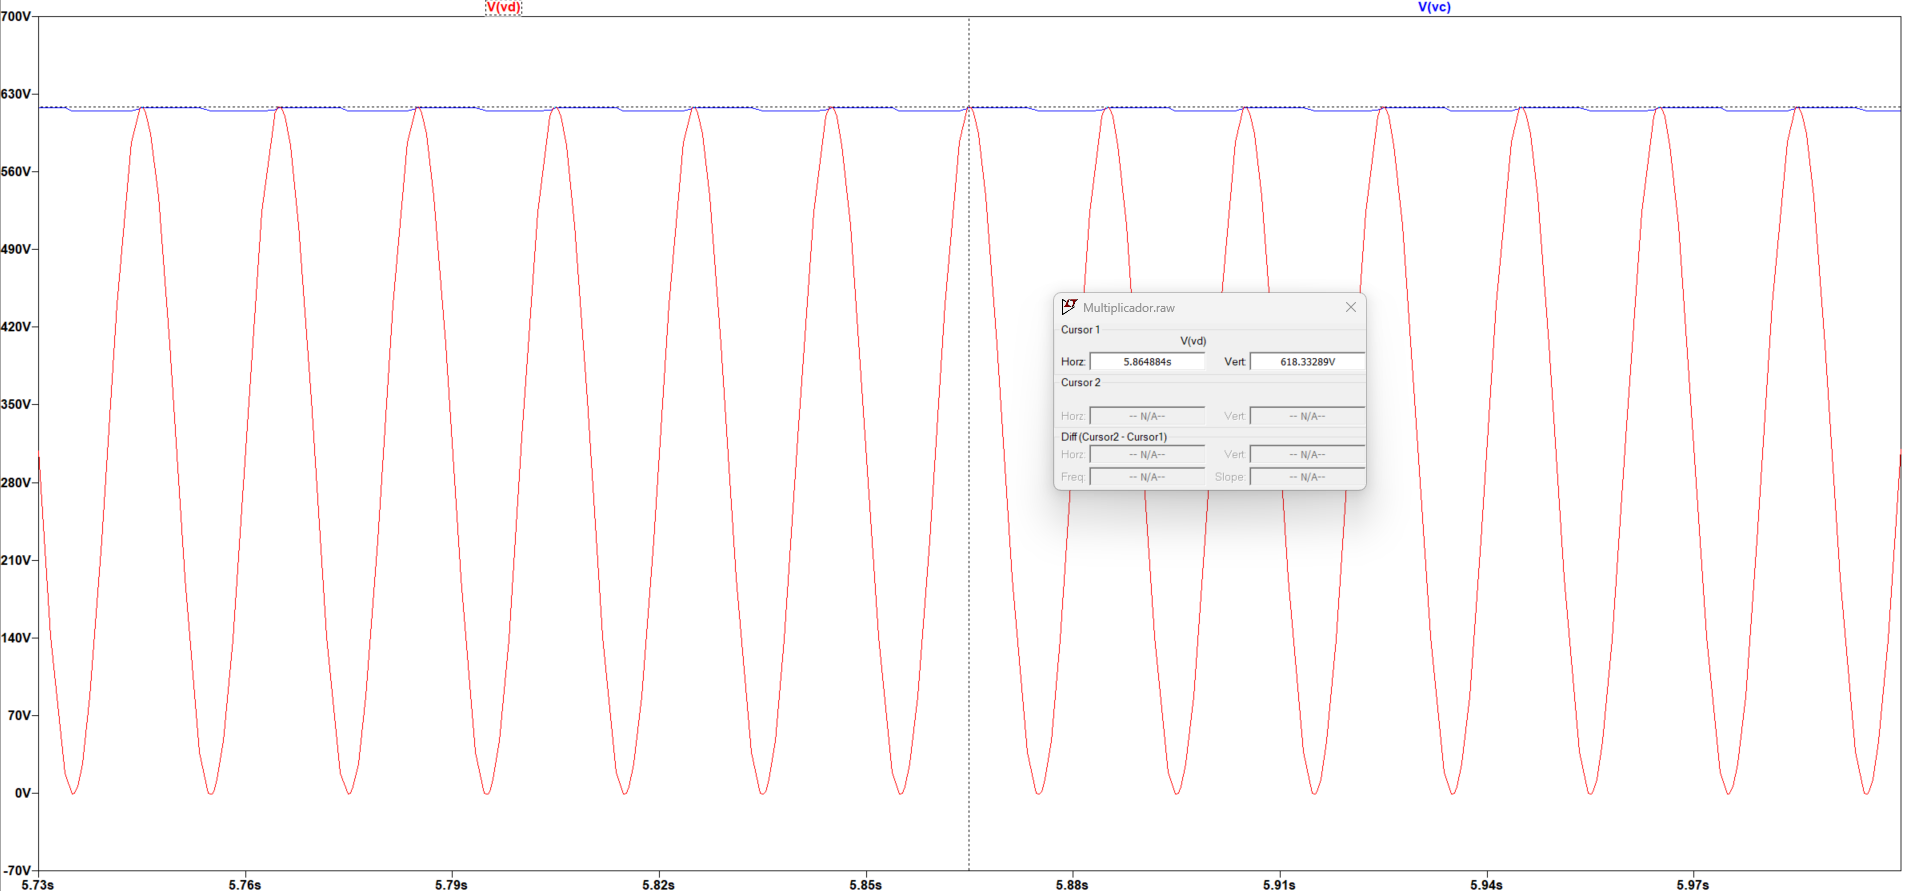
\includegraphics[width=1\textwidth]{Imagenes_alvaro/Vmax.png}
    \caption{Tensión máxima en condensadores y diodos}
    \label{Vmax}
\end{figure}

También es necesario comprobar que la tensión en el multímetro no supera los $200V$ establecidos. Puesto que se definió el divisor para obtener $200V$
para la máxima tensión de salida posible ($3111,27V$), en este caso la tensión medida será necesariamente menor, dando un valor de $195,91V$ como se puede ver en la figura
\ref{V_mult}.

\begin{figure}[H]
    \centering
    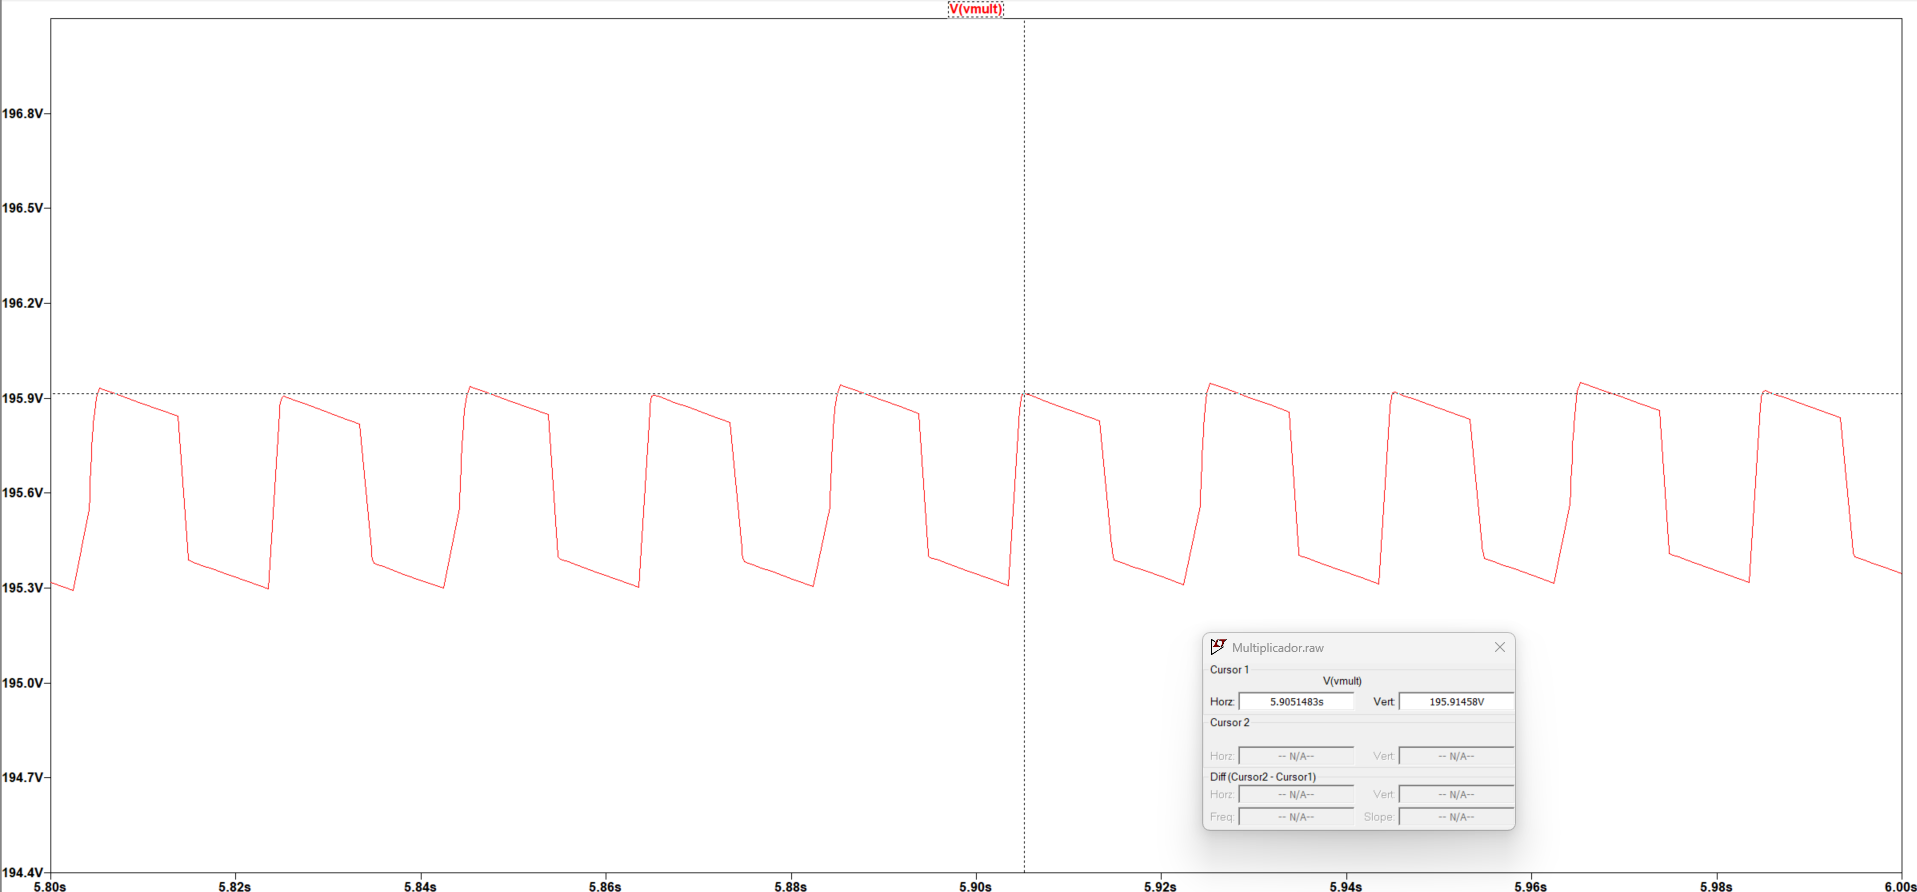
\includegraphics[width=1\textwidth]{Imagenes_alvaro/V_mult.png}
    \caption{Tensión en el multímetro}
    \label{V_mult}
\end{figure}

En la figura \ref{200hz} se puede ver la tensión de salida y corriente de carga a $50Hz$ (gráfica roja), $100Hz$ (gráfica azul), $150Hz$ (gráfica verde)
y $200Hz$ (gráfica azul claro). Como se ha calculado previamente la tensión obtenida aumenta con la frecuencia, lo que produce un aumento de la corriente en consecuencia.
Se obtiene una tensión de salida de $3090V$ y una corriente de carga de $4,963mA$ para una frecuencia de $200Hz$. Obtenemos los errores respecto a los valores esperados:

\begin{equation}
    E_{V_{load-200Hz}} = \frac{3095,44V - 3090V}{3095,44V} \cdot 100 = 0,18\%
\end{equation}

\begin{equation}
    E_{I_{load-200Hz}} = \frac{5mA - 4,963mA}{5mA} \cdot 100 = 0,74\%
\end{equation}

\begin{figure}[H]
    \centering
    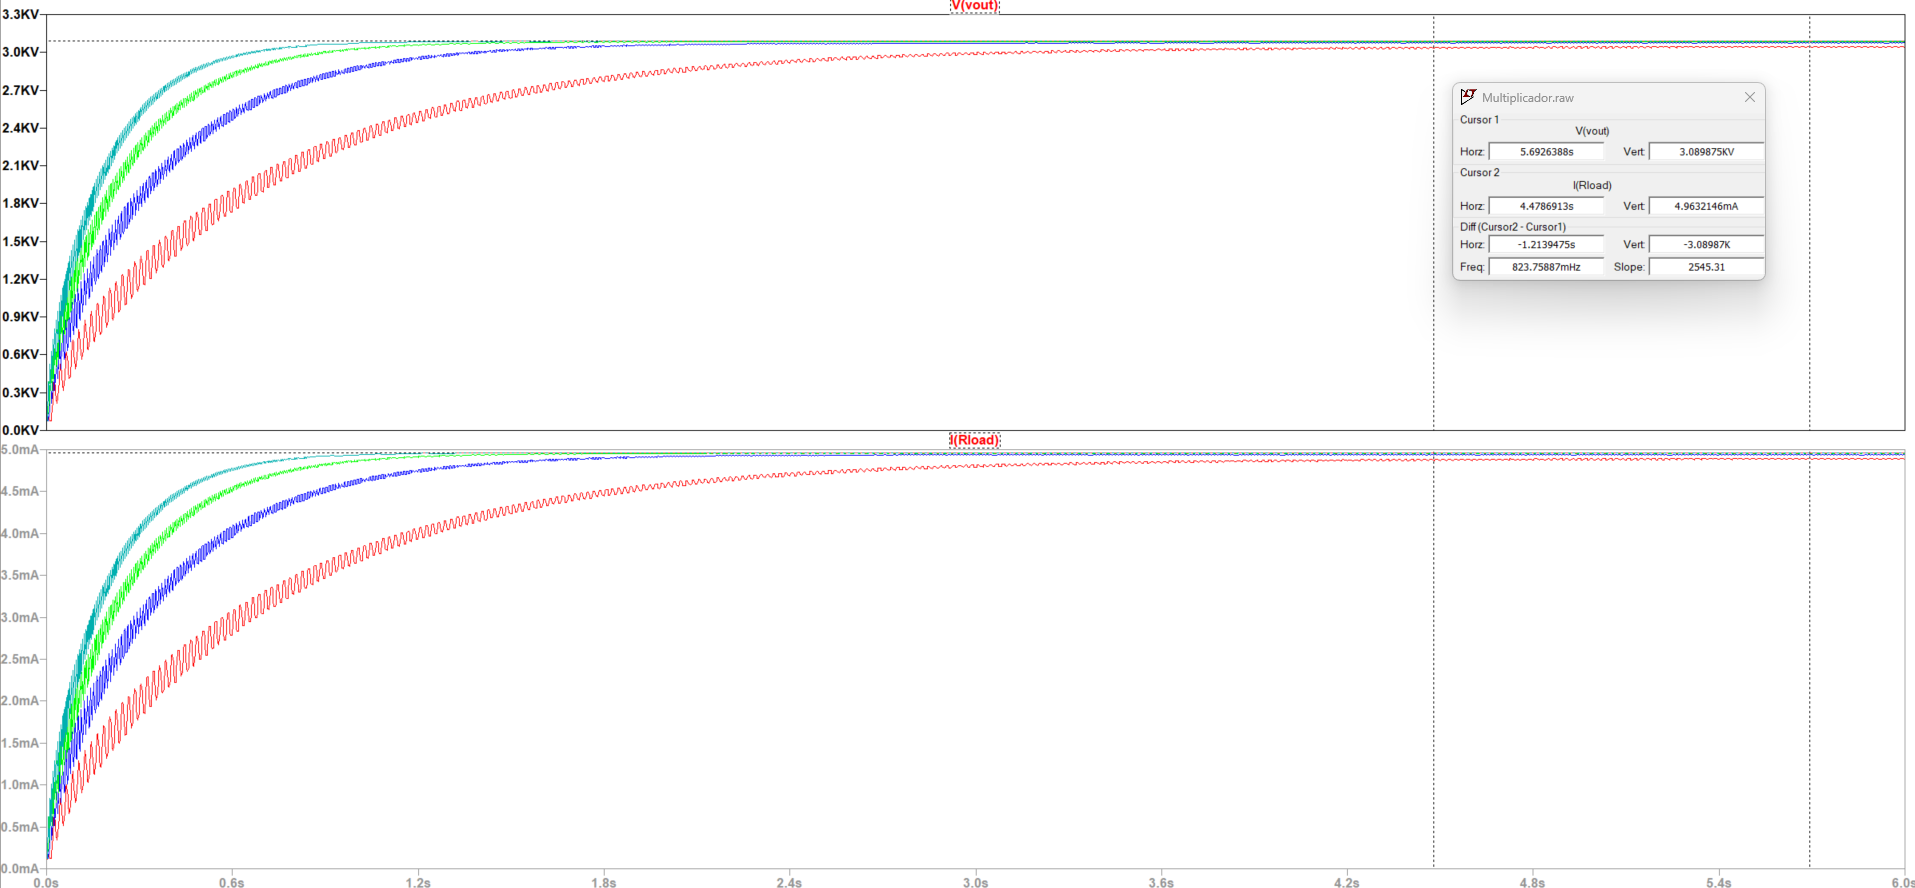
\includegraphics[width=1\textwidth]{Imagenes_alvaro/200hz.png}
    \caption{Tensión de salida y corriente en la carga para múltiples frecuencias}
    \label{200hz}
\end{figure}

Finalmente, se comprueba al funcionamiento del circuito para una señal de entrada cuadrada de $50Hz$, con valores máximos y mínimos iguales a los valores
de pico positivo y negativo de la senoidal y con un ciclo de trabajo del $50\%$. El resultado se puede ver en la figura \ref{cuadrada}, donde se obtiene
un valor medio de $3044V$, exactamente igual que el obtenido con la senoidal de misma frecuencia. También se mantiene el mismo rizado de $10V$ del caso anterior.

\begin{figure}[H]
    \centering
    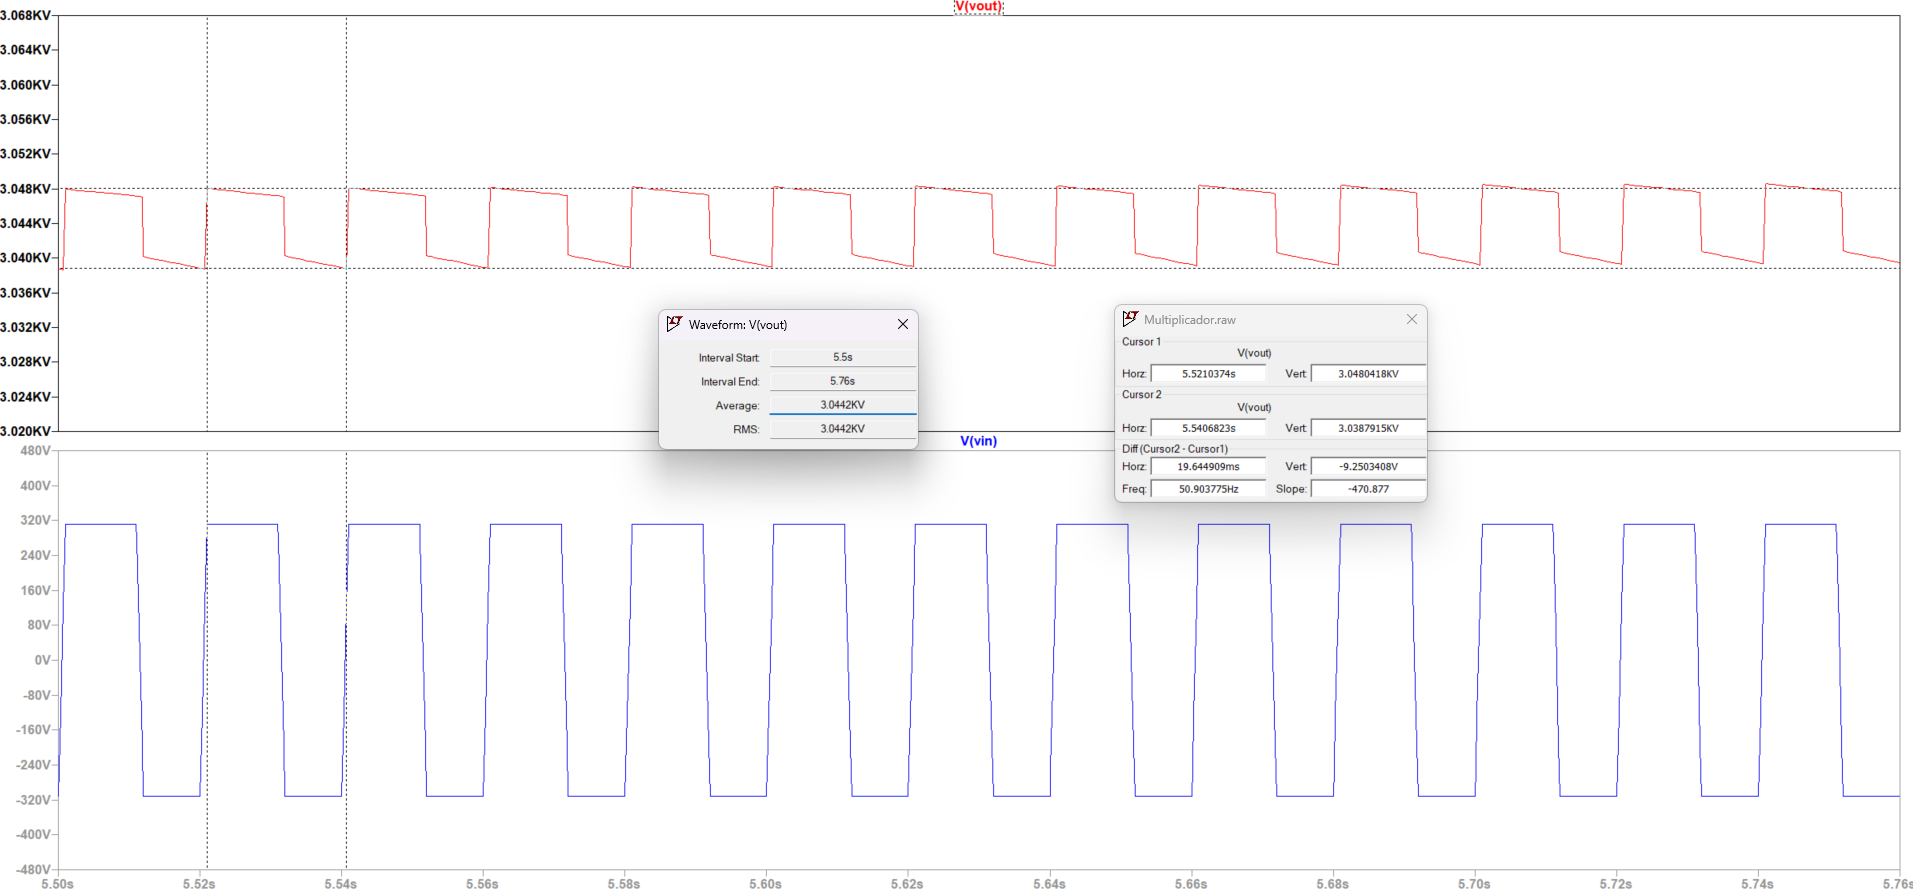
\includegraphics[width=1\textwidth]{Imagenes_alvaro/cuadrada.png}
    \caption{Tensión de salida y entrada con señal de entrada de onda cuadrada}
    \label{cuadrada}
\end{figure}

\section{Conclusiones}

En esta práctica se ha llevado a cabo el diseño y simulación de un 
circuito Multiplicador de Greinacher capaz de proporcionar a la salida 
$3kV$ a partir de una fuente de $220V$, asegurando un adecuado suministro de 
corriente sin un rizado y caída de tensión significativo. Para lograrlo se ha realizado 
un dimensionamiento de los condensadores a partir de un valor seleccionado de rizado de pico a 
pico máximo igual a $10V$.

Por otro lado, se ha diseñado un circuito sencillo de medida de tensión a partir de un divisor 
de tensión de tal forma que se puede medir la tensión de salida del multiplicador en un fondo 
de escala de $200V$.

Además, en las simulaciones se ha podido comprobar el correcto funcionamiento del circuito y la fiabilidad 
de los cálculos teóricos, los cuales han proporcionado aproximaciones con poco error.

Con los resultados obtenidos se puede destacar el atractivo de este tipo de soluciones para conseguir 
una elevada tensión a partir de una estructura sencilla basada en diodos y condensadores para aplicaciones 
que requieran de una elevada tensión sin la complejidad de circuitos conmutados o transformadores. También se 
destaca la funcionalidad del multiplicador diseñado, el cual ha demostrado ser apto para un amplio rango 
de frecuencias (de $50Hz$ a $200Hz$) y para una señal senoidal y cuadrada.

Por el contrario, estos circuitos presentan ciertas limitaciones que deben considerarse. En aplicaciones con 
cargas altamente variables, la caída de tensión resultante puede afectar a su rendimiento. Asimismo, su empleo puede 
ser complicado en aplicaciones 
con mucha variación de la frecuencia, especialmente cuando la frecuencia es demasiado baja. Otro inconveniente es el tiempo de carga relativamente lento, lo que puede 
ser problemático en sistemas que requieran una respuesta rápida en la elevación de la tensión. Por último, este tipo 
de circuitos suelen estar restringidos a aplicaciones de baja potencia, ya que su capacidad 
de suministrar corriente es limitada.

